\documentclass[svgnames] {beamer}
\usepackage{cmlgc}
\usepackage{comment}
\usepackage{tikz}
\usefonttheme{serif}     % Font theme: serif
\usepackage[T2A]{fontenc}
\usepackage[utf8]{inputenc}
\usepackage[english,russian]{babel}
\usepackage{amssymb,amsfonts,amsmath,mathtext,cite,enumerate,float} %подключаем нужные пакеты расширений
% \usepackage{cyrillic}
\usepackage{color, colortbl}
\usepackage{multirow}
\usepackage{graphicx}
\usepackage{graphics}
\usepackage{multirow}
\usepackage{url}
\usepackage{hyperref}
\usepackage{animate}


\usepackage{ragged2e} %выравнивание текста по ширине слайда (\justifying)
%\setbeamercolor{background canvas}{bg=violet}

\usetheme{AnnArbor}
\usecolortheme{crane}

%=================================================

    \defbeamertemplate*{footline}{mytheme}{%
      \leavevmode%
      \hbox{%
      \begin{beamercolorbox}[wd=.2\paperwidth,ht=3ex,dp=1ex,center]{author in head/foot}%
        \usebeamerfont{author in head/foot}\insertshortauthor
      \end{beamercolorbox}%
      \begin{beamercolorbox}[wd=.7\paperwidth,ht=3ex,dp=1ex,center]{title in head/foot}%
        \usebeamerfont{title in head/foot}\insertshorttitle
      \end{beamercolorbox}%
      \begin{beamercolorbox}[wd=.1\paperwidth,ht=3ex,dp=1ex,right]{date in head/foot}%
        %\usebeamerfont{date in head/foot}\insertshortdate{}\hspace*{2em}
        %\insertframenumber{} / \inserttotalframenumber\hspace*{2ex} %номер текущего слайда / общее число слайдов
        \insertframenumber{} \hspace*{5ex}  %номер текущего слайда
      \end{beamercolorbox}}%
      \vskip0pt%
    }
    \usebeamertemplate{mytheme}


\defbeamertemplate*{frametitle}{boldTitle}{%
    \begin{beamercolorbox}[wd=\paperwidth,ht=3ex,dp=3pt,left]{title in head/foot}%
%        \ \textit{\textbf{\insertframetitle}} % курсивный заголовок слайда 
        \ \textbf{\insertframetitle}
    \end{beamercolorbox}
}
\usebeamertemplate{boldTitle}

%=================================================
% \titlegraphic{
\includegraphics[width=\textwidth]{logo_conf.png}}
\addtobeamertemplate{title page}{
\includegraphics[scale=0.39]{logo_conf.png}}{}
\title[Экстраполяция карты магнитного поля дипольного магнита SP-41 эксперимента BM@N ...]{\textbf{\large {Экстраполяция карты магнитного поля дипольного магнита SP-41 эксперимента BM@N на Нуклотроне ОИЯИ}}}

\author[П. Батюк]{\textit{\textbf{{\footnotesize \underline{П.~Батюк}, С.~Мерц, О.~Рогачевский}}}}
\institute{\url{batyuk@jinr.ru}  \\ Лаборатория Физики Высоких Энергий, ОИЯИ}

%\date{{\textbf{Международная молодёжная конференция \\ \color{blue} ``Современные проблемы прикладной математики и информатики''} \\ 
% \newpage \footnotesize Ноябрь 17 - 21, 2014}}

      
\begin{document}
\maketitle

% Slide #1b
\begin{frame}
  \frametitle{\centering Экстраполяция карты ... }
  \begin{block}{\textbf {\centering План доклада:}}
    %\newline
    \begin{enumerate}
    \item \textbf {Магнит и существующая карта магнитного поля} 
      \newline
    \item \textbf {Обоснование необходимости экстраполяции} 
      \newline
    \item \textbf {Подход, используемый для экстраполяции}
      \newline
    \item \textbf {Полученные результаты}
    \end{enumerate}
  \end{block}
\end{frame}

% Slide #1b
\begin{frame}
 \frametitle{Актуальная геометрия эксперимента BM@N}
 \begin{center}
   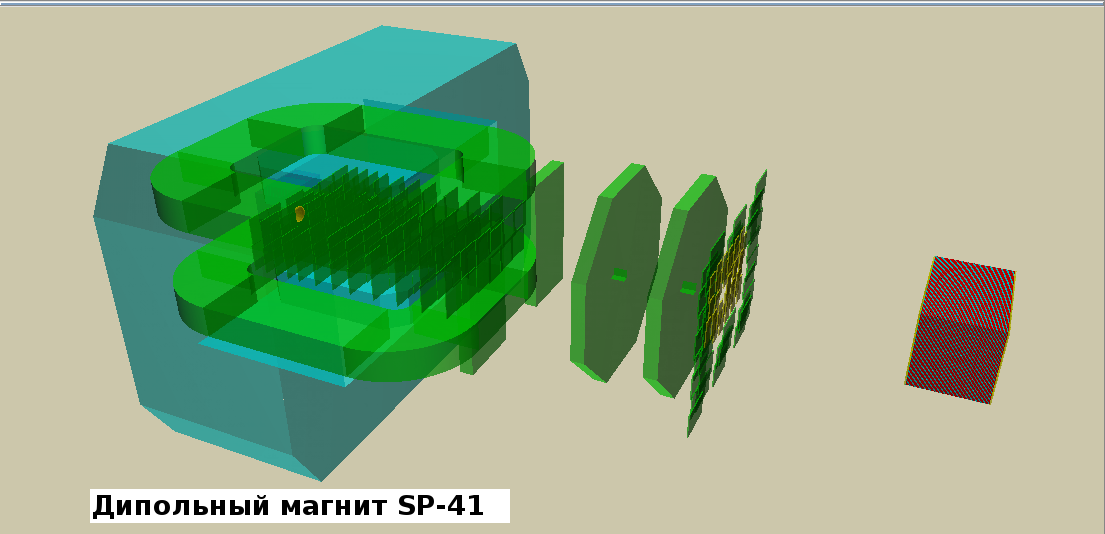
\includegraphics[width=1.0\linewidth]{bmn_genView.png}
 \end{center}
\end{frame}

% Slide #1a
\begin{frame}
  \frametitle{Магнит SP-41, общий вид}
  \begin{center}
  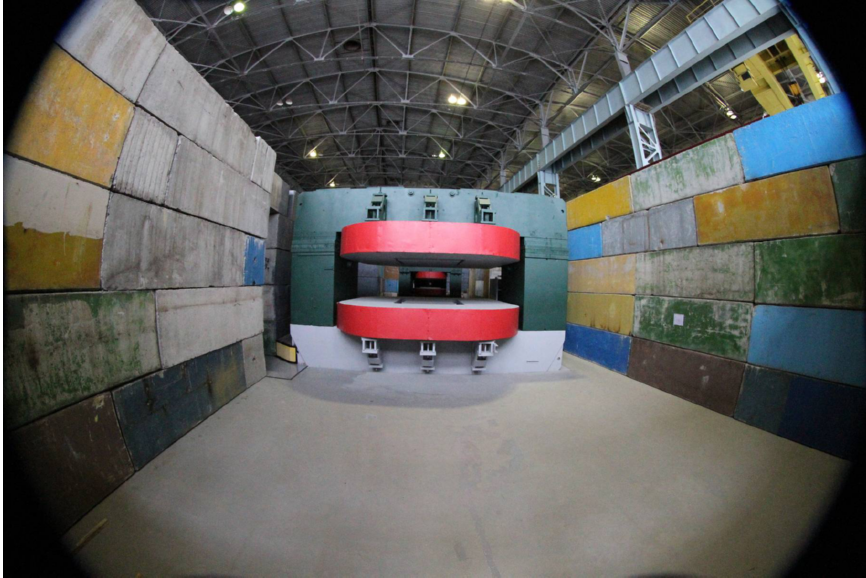
\includegraphics[width=0.8\linewidth]{sp41_genView.png}
  \end{center}
\end{frame}

% Slide #1
\begin{frame}
  \frametitle{Магнит SP-41, система координат}
  % \begin{columns}[c]
  %   \column{.6\textwidth}
  \begin{block}{}
    \begin{figure}[H]
      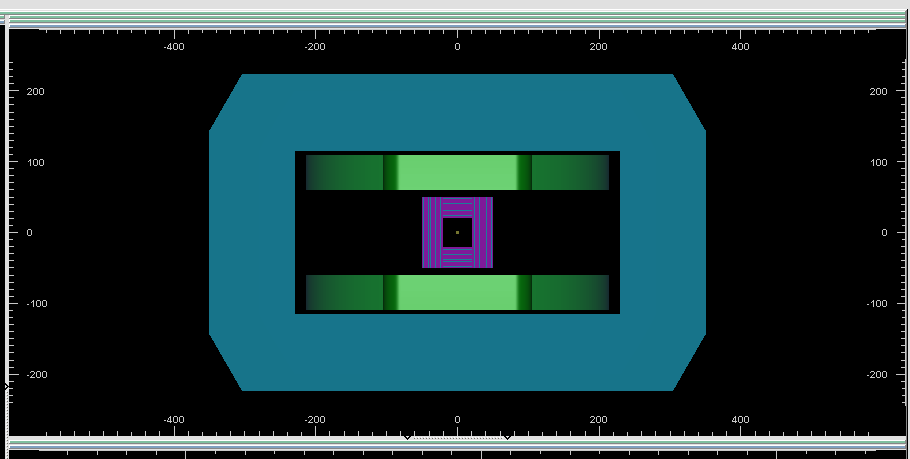
\includegraphics[width=0.8\linewidth]{bmn_magnetGeom.png}
    \end{figure}
  \end{block}
  %    \column{.4\textwidth}
  \begin{block}{\centering \bf Область карты магнитного поля:}
    \begin{center}
      $|X| \leq 228 $ см \\
      $|Y| \leq 54 $ см \\
      $0 \leq  Z \leq 322.5$ см
    \end{center}
  \end{block}
  %  \end{columns}
\end{frame}

% Slide #2
\begin{frame}
  \frametitle{Использование карты магнитного поля}
  \begin{columns}[c]
    \column{.3\textwidth}
    \begin{block}{\centering \bf Формат карты}
      \centering 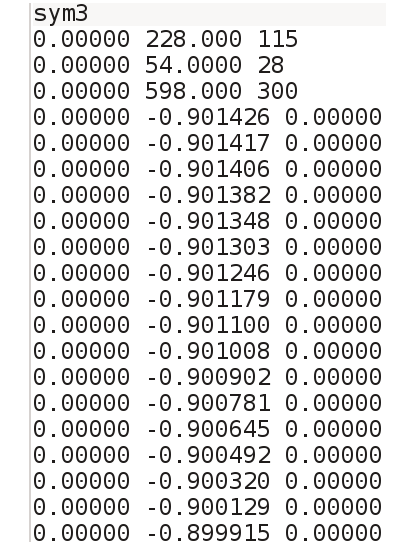
\includegraphics[width=1.0\linewidth]{magFieldMap_format.png}
    \end{block}
    \column{.6\textwidth}
    \begin{block}{\centering \bf Взятие поля в конкретной точке}
      \centering fieldMap->GetBx(x, y, z);
      \centering fieldMap->GetBy(x, y, z);
      \centering fieldMap->GetBz(x, y, z);
    \end{block}
    \begin{block}{sym3:}
      \centering $x > 0, ~ y > 0, ~ z > 0$ \\
      \begin{itemize}
      \item { \bf $B_{x}$ антисимметрична по $x$ и симметрична по $y$ и $z$} \\
      \item { \bf $B_{y}$ симметрична по $x$, $y$ и $z$} \\
      \item { \bf $ B_{z}$ антисимметрична по $x$ и $z$ и симметрична по $y$}
      \end{itemize}
    \end{block}
  \end{columns}
\end{frame}

%% Slide #3a
\begin{frame}
  \frametitle{\centering Обоснование необходимости экстраполяции}
  \begin{block}{\centering \bf Исходная карта поля, $Y = 0$}
    \centering 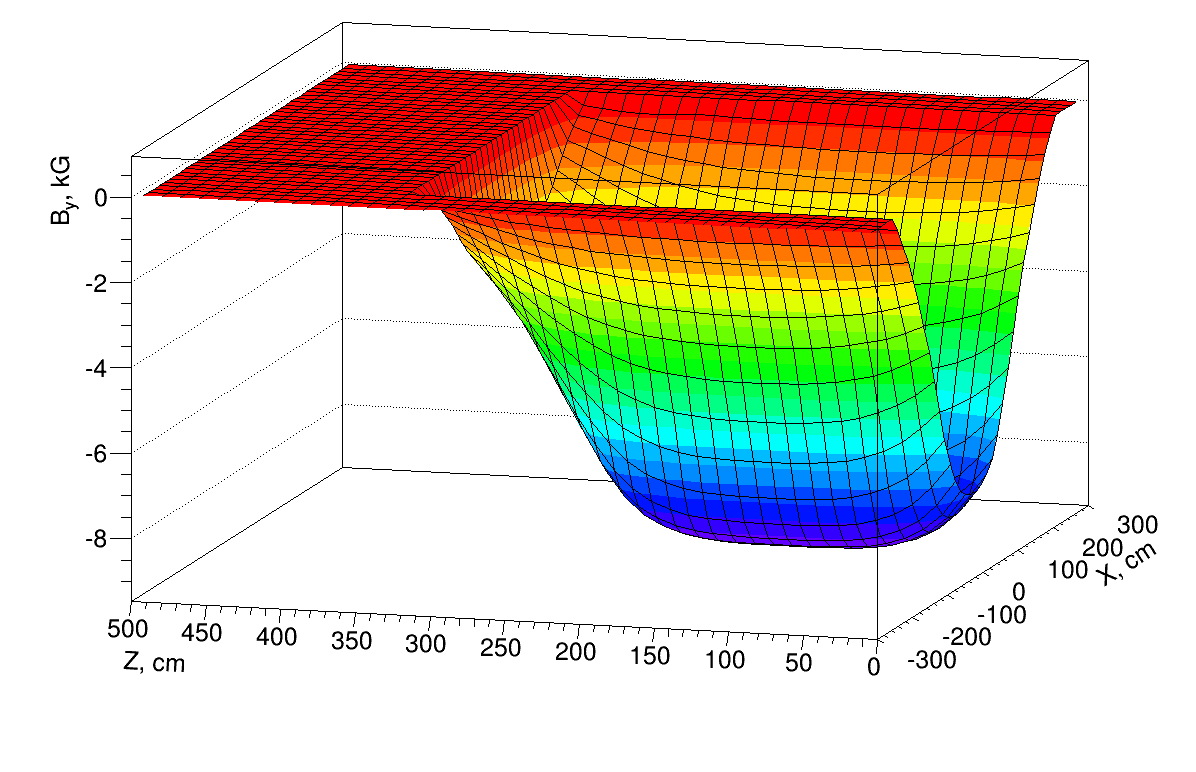
\includegraphics[width=1.0\linewidth]{fieldMap_orig_pic2.png}
  \end{block}
\end{frame}

% Slide #3
\begin{frame}
  \frametitle{Обоснование необходимости экстраполяции}
  \begin{block}{}
    \centering 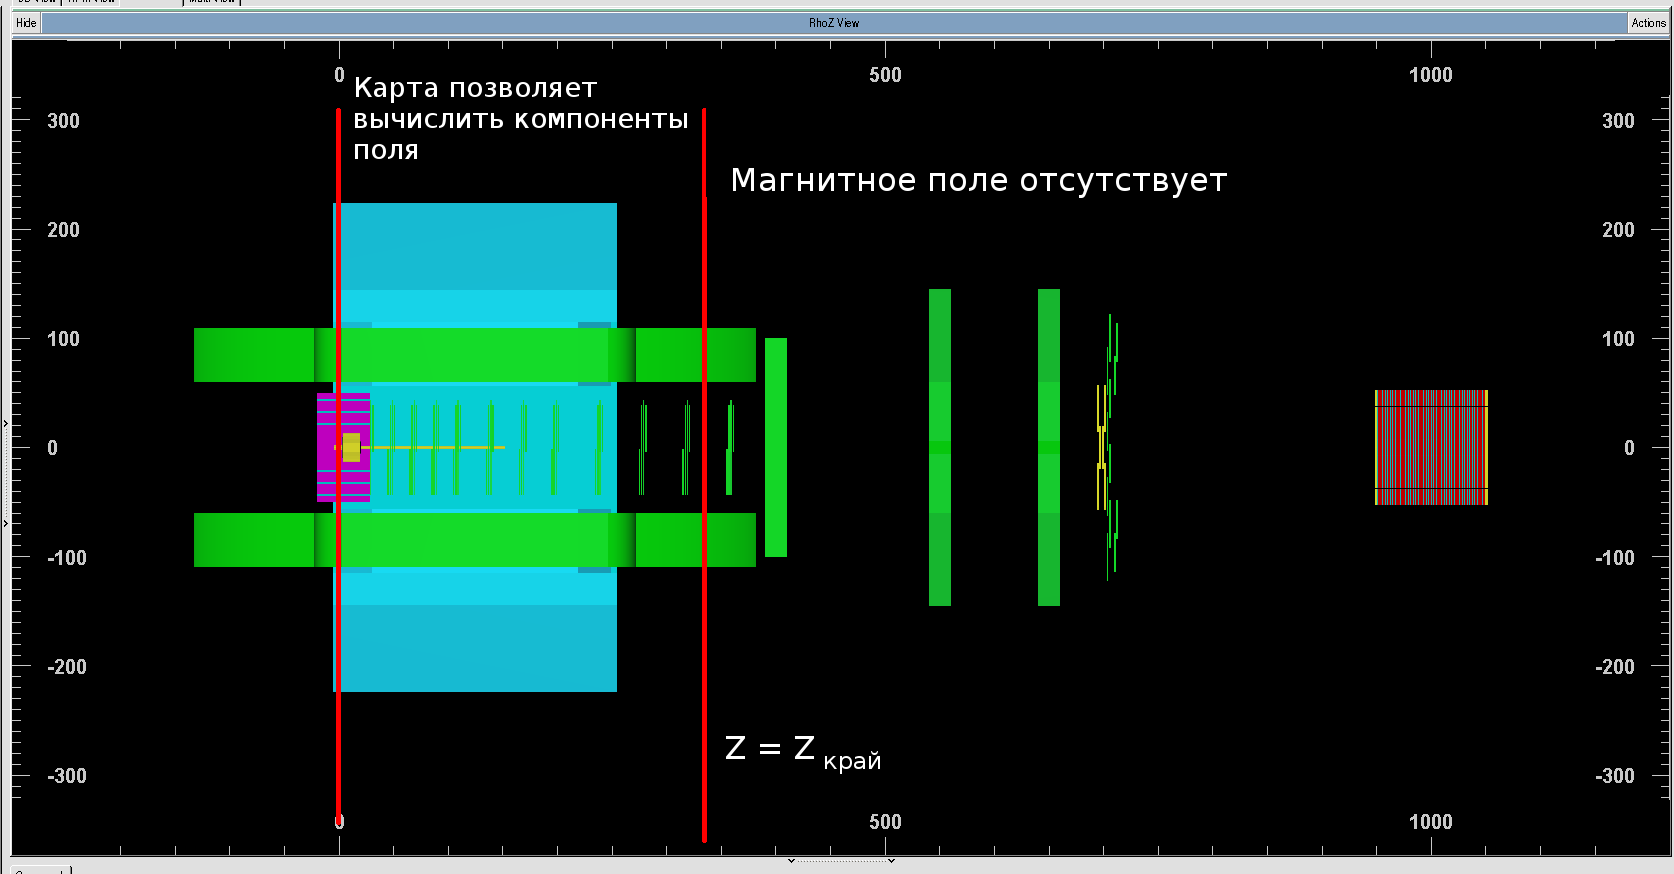
\includegraphics[width=0.8\linewidth]{extrap_explan.png}
  \end{block}
  \begin{block}{}
    \begin{itemize}
    {\footnotesize \item  \bf При Z = $Z_{edge}$ магнитное поле не становится равным нулю.}
    {\footnotesize \item  \bf Информация о координате $Z$, начиная с которой можно считать магнитное поле равным нулю, является крайне критичной.}
    \end{itemize}
  \end{block}
\end{frame}

% Slide #4a
\begin{frame}
  \frametitle{Используемый подход}
  \begin{block}{\bf \centering Требования к используемым функциям:}
    \begin{itemize}
      \item {\bf Гладкость (непрерывная дифференцируемость);}
        \begin{itemize}
        \item Возможность найти значение в любой точке области экстраполяции;
        \end{itemize}
      \item {\bf Монотонность};
        \begin{itemize}
        \item Характер поведения экстраполируемой компоненты не должен меняться;
        \end{itemize}
      \item {\bf Ограниченность};
        \begin{itemize}
        \item Знак компоненты не должен меняться;
        \end{itemize}
    \end{itemize}
  \end{block}
%  \begin{block}{}
%    \begin{center}
%    \bf Интерполяционные полиномы не подходят
%    \end{center}
%  \end{block}
\end{frame}


% Slide #4
\begin{frame}
  \frametitle{Используемый подход}
  \begin{block}{\centering \bf Общий вид функций}
    \begin{equation}
      B_{comp}(x, y, z) = C(x, y) \cdot e^{-\frac{(z - \mu(x,y))^{2}}{2 \sigma(x,y)^{2}}}
      \label{form1}
    \end{equation}
    \begin{equation}
      \lim_{z \to \infty} B_{comp}(x, y, z) = 0
      \label{form2}
    \end{equation}
  \end{block}
  \begin{block}{}
    \begin{enumerate}
      {\footnotesize \item \bf На плоскости XoY (|X| < $X_{max}$ и |Y| < $Y_{max}$) строилась равномерная сетка размерности $N \cdot N$ узлов.} 
      {\footnotesize \item \bf В каждом узле сетки для диапазона Z = [260 .. 320] см проводилась аппроксимация компоненты магнитного поля  функцией (\ref{form1}).}
      {\footnotesize \item \bf Аппроксимация для каждого узла сетки позволяет получить три дискретно заданные функции  для определения коэффициентов $C(x, y)$, $\mu(x, y)$ и $\sigma(x, y)$.}
      {\footnotesize \item \bf Используя билинейную интерполяцию, оцениваются значения коэффициентов в произвольной точке с координатами (x, y) 
        для дальнейшего использования в формуле (\ref{form1}).}
    \end{enumerate}
  \end{block}
\end{frame}

% Slide #5
\begin{frame}
  \frametitle{Используемый подход}
  \begin{block}{\centering \bf Аппроксимация компоненты поля функцией вида (\ref{form1})}
    \centering 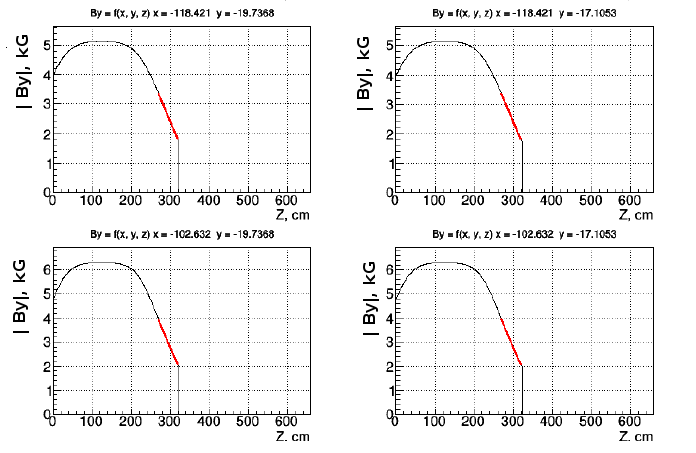
\includegraphics[width=0.6\linewidth]{gauss_fitting.png}
  \end{block}
\end{frame}

% Slide #5
\begin{frame}
  \frametitle{Проверка качества экстраполяции}
  \begin{block}{\centering \bf $Z = 300 ~..~ 316$ см, компонента $B_{x}$}
    \begin{columns}[c]
      \column{.45\textwidth}
      \begin{block}{\centering Карта поля}
        \centering 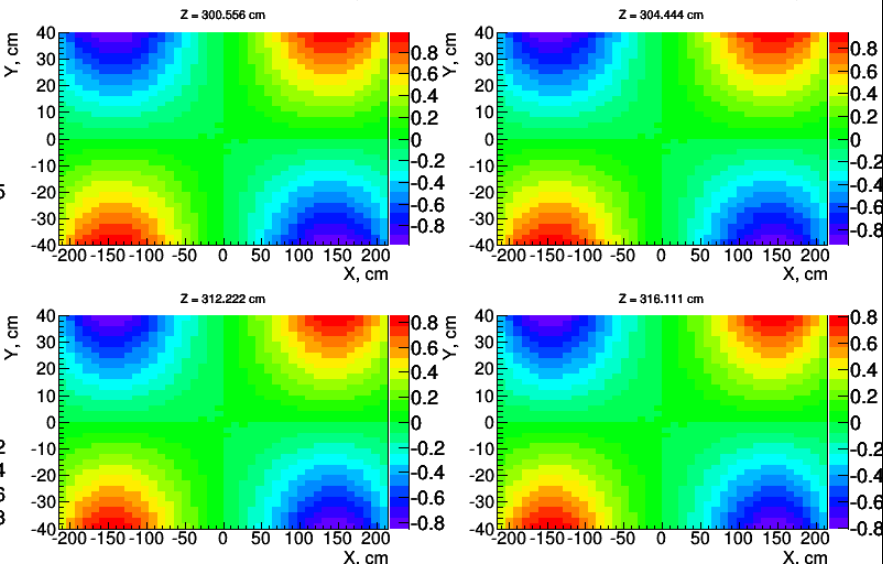
\includegraphics[width=1.0\linewidth]{Bx_fieldMap_new.png}
      \end{block}
      \column{.45\textwidth}
      \begin{block}{\footnotesize Относительная погрешность \centering $\delta$, \%}
        \centering 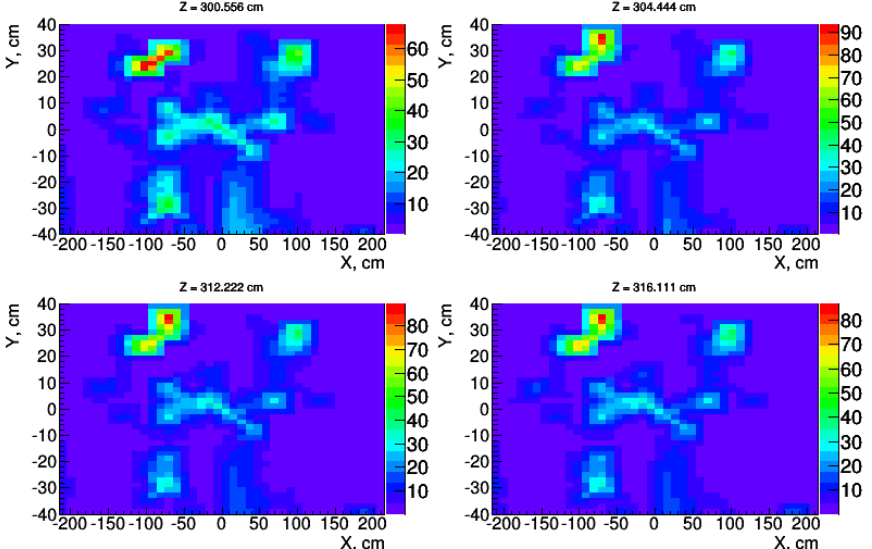
\includegraphics[width=1.0\linewidth]{Bx_diff_overlap_reg_new.png}
      \end{block}
    \end{columns}
   \end{block} 
 \end{frame}

% Slide #5
\begin{frame}
  \frametitle{Проверка качества экстраполяции}
  \begin{block}{\centering \bf $Z = 300 ~..~ 316$ см, компонента $B_{y}$}
    \begin{columns}[c]
      \column{.45\textwidth}
      \begin{block}{\centering Карта поля}
        \centering 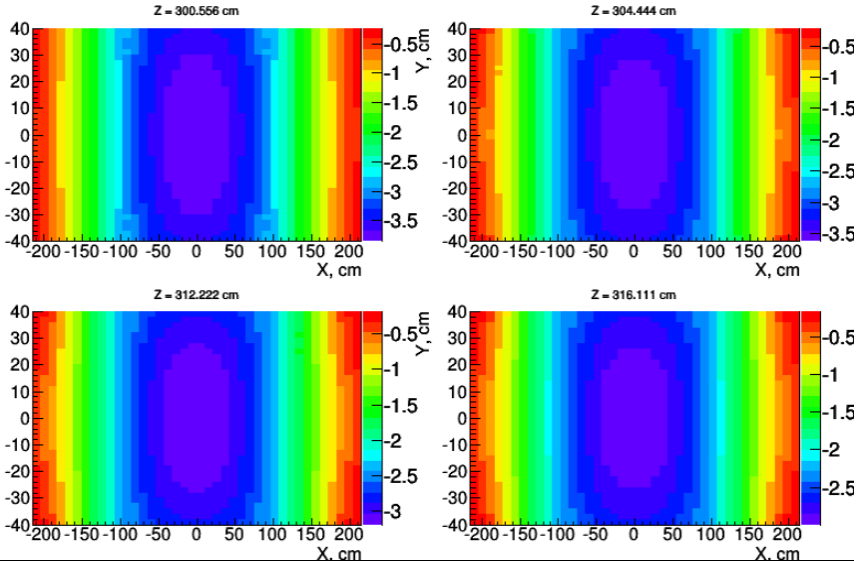
\includegraphics[width=1.0\linewidth]{By_fieldMap_new.png}
      \end{block}
      \column{.45\textwidth}
      \begin{block}{\footnotesize Относительная погрешность \centering $\delta$, \%}
        \centering 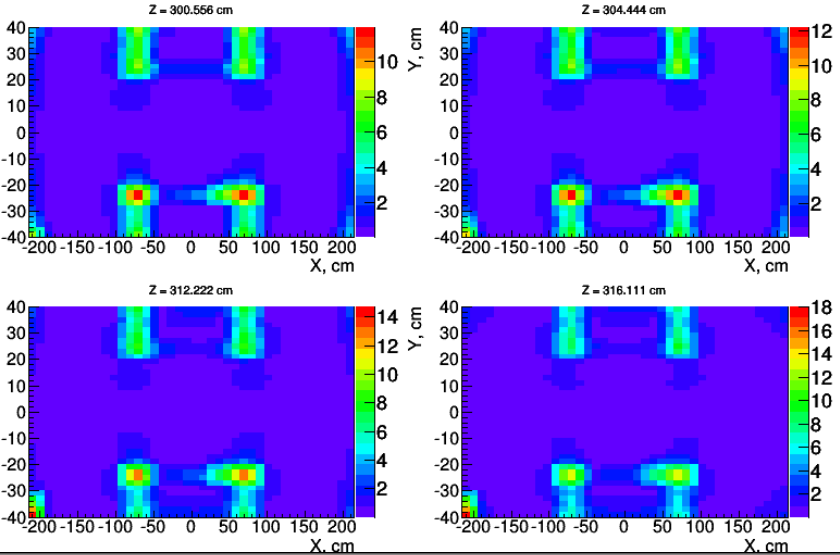
\includegraphics[width=1.0\linewidth]{By_diff_overlap_reg_new.png}
      \end{block}
    \end{columns}
   \end{block}  
\end{frame}

% Slide #5
\begin{frame}
  \frametitle{Проверка качества экстраполяции}
  \begin{block}{\centering \bf $Z = 300 ~..~ 316$ см, компонента $B_{z}$}
    \begin{columns}[c]
      \column{.45\textwidth}
      \begin{block}{\centering Карта поля}
        \centering 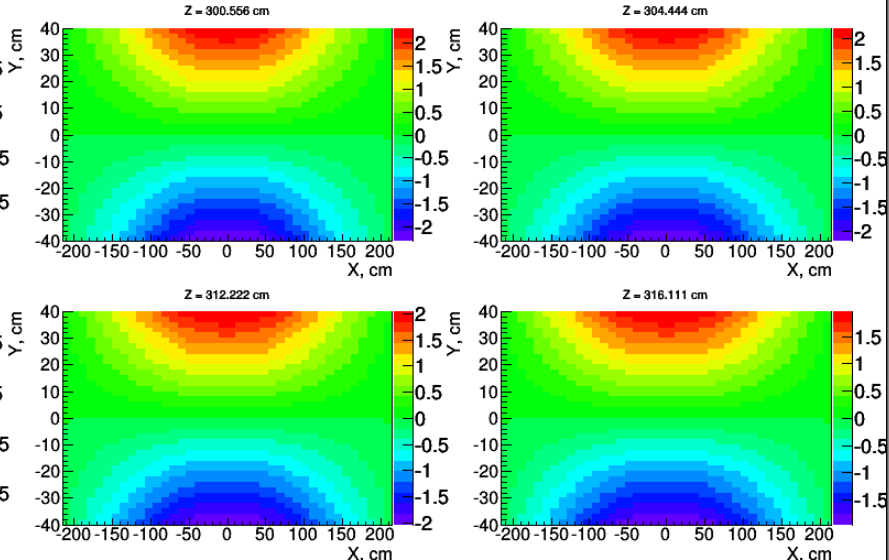
\includegraphics[width=1.0\linewidth]{Bz_fieldMap_new.png}
      \end{block}
      \column{.45\textwidth}
      \begin{block}{\footnotesize Относительная погрешность \centering $\delta$, \%}
        \centering 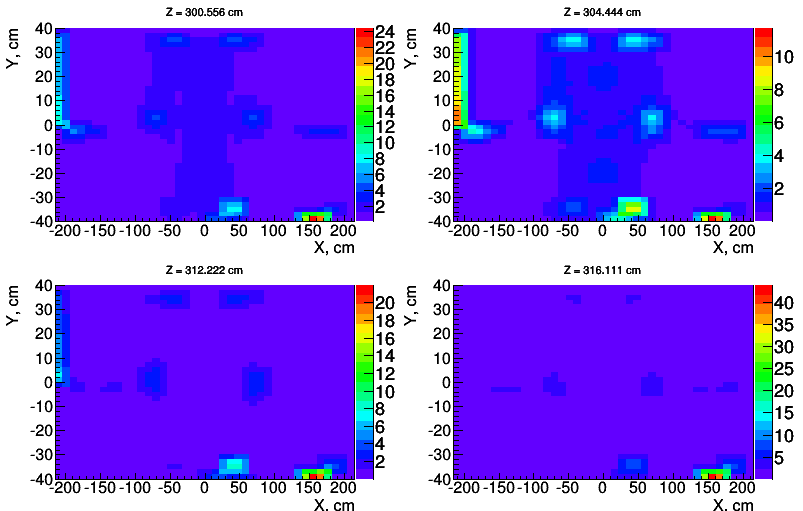
\includegraphics[width=1.0\linewidth]{Bz_diff_overlap_reg_new.png}
      \end{block}
    \end{columns}
  \end{block} 
\end{frame}

% Slide #5a
\begin{frame}
  \frametitle{Проверка качества экстраполяции}
   \begin{block}{\centering \bf Экстраполированная карта поля, $Y = 0$}
      \centering 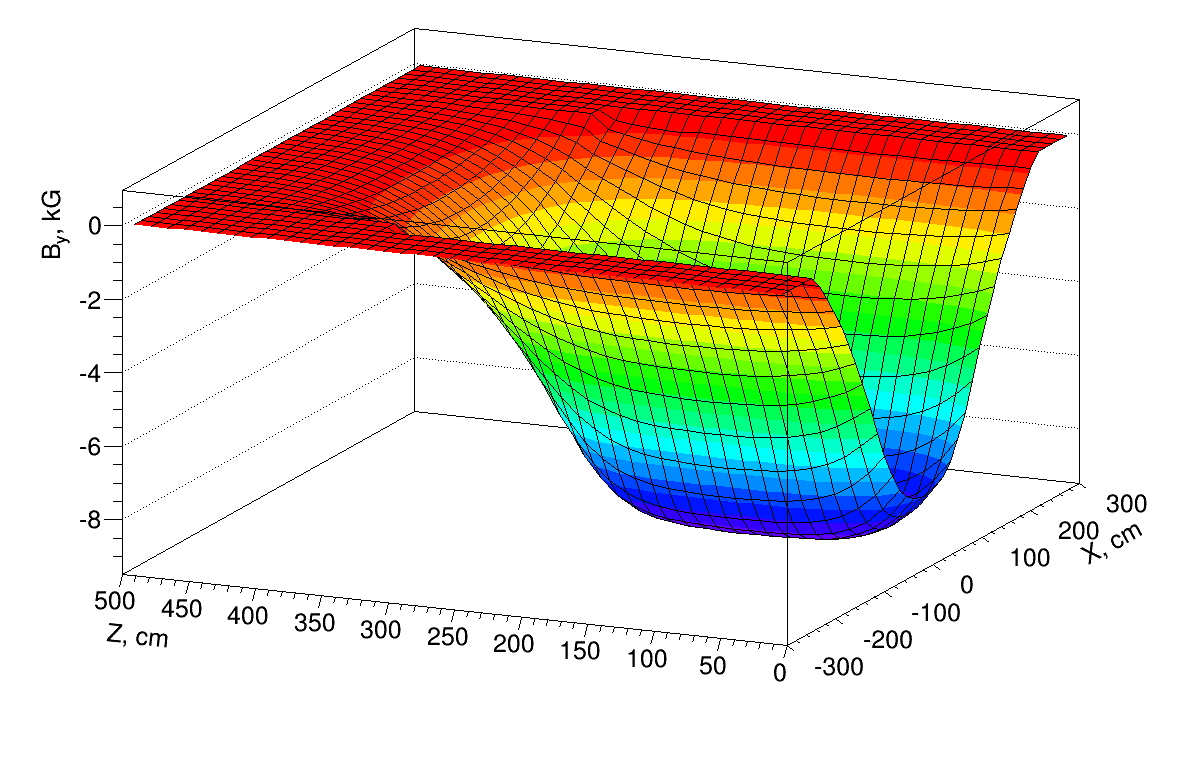
\includegraphics[width=1.0\linewidth]{fieldMap_extrap_pic2.png}
    \end{block}
 \end{frame}

% Slide #6
\begin{frame}
  \frametitle{Результаты}
  \begin{enumerate}
  \item \bf Предложен и реализован подход, позволяющий осуществить качественную и эффективную экстраполяцию магнитного поля за пределы области карты.
  \item \bf В результате анализа выявлены проблемные зоны внутри карты магнитного поля, требующие проведения новых более тщательных измерений. 
  \item \bf Результаты расчета внедрены в программный комплекс BmnRoot.
  \item \bf \color{red}Планируется осуществить анализ эффективности глобального трекинга с использованием расширенной карты поля.
  \end{enumerate}
 \end{frame}


%%%%%%%%%%%%%%%%%%%





\begin{comment}

%%%%% Slide #1

\begin{frame}
  \frametitle{Plan of research work}
  \begin{block}{\textbf {The Research Work consists of the following basic stages:}}
   %\newline
    \begin{enumerate}
   	\item \textbf {Analysis of residuals depending on $(\phi, \theta)$-angles} 
		\newline
                 \item \textbf {Analysis of Edge Effects} 
                 \newline
                 \item \textbf {Normalization of errors obtained from the algorithm}
                 \newline
                  \item \textbf {Preliminary results on the Particle Momentum Resolution}
    \end{enumerate}
  \end{block}
\end{frame}

\begin{frame}
	\frametitle{MPD and TPC} \label{goBack}
	{\tiny	
	\begin{figure}[H]
		\centering
		\begin{minipage}[h]{0.45\linewidth}
		\center{Detector MPD\\ \includegraphics[width=0.8\linewidth]{mpd_new.png}}
		\end{minipage}
		\vrule
		\begin{minipage}[h]{0.45\linewidth}
		\center{Time Projection Chamber TPC\\ \includegraphics[width=0.8\linewidth]{tpcscheme.png}}
		\end{minipage}
		\hrule
		\vfill
		\begin{minipage}[h]{0.45\linewidth}
		\center{Principle of operation of TPC\\ \includegraphics[width=0.8\linewidth]{TPC_work.png}}
		\end{minipage}
		\vrule
		\begin{minipage}[h]{0.45\linewidth}
		\center{Scheme of read-out sector \\ \includegraphics[width=0.7\linewidth]{tpc_sector.png}}
		\end{minipage}
	\end{figure}
	}
\end{frame}


\begin{frame}
	\frametitle{Reconstruction algorithm of responses of TPC ...}
	\begin{block}{... consists of three stages:}
		\begin{enumerate}
			%\item Поиск обобщенных кластеров в пространстве <<Пэд-Время>> для каждой строки пэдов.
			\item Search of extended clusters in the space <<Pad-Time>> for each padrow
			%\item Поиск пиков во временном профиле для каждого пэда в обобщенном кластере.
			\item Search of peaks in the time profile in the extended cluster
			%\item Группировка соседних пиков в хиты и вычисление их координат.
			\item Merging of the neighbouring peaks into hits to make a subsequent calculation of their coordinates
		\end{enumerate}
	\end{block}
\end{frame}

%\begin{comment}
\begin{frame}
	\frametitle{Формирование итоговых хитов}
	\centering
	{\tiny	
	\begin{columns}[t]
		\column{.55\textwidth}
		\begin{block}{}
		\centering Пример распределения обобщенных кластеров
		\end{block}
		\begin{center}
			\includegraphics[width=1.0\linewidth]{extClustersUrQMD.png}
		\end{center}
		\column{.35\textwidth}
		\begin{block}{}
			\centering Схематический вид алгоритма заливки
		\end{block}
		\begin{center}
			\animategraphics[controls, height=5cm]{1}{flood-fill_}{0}{18} 
		\end{center}
	\end{columns}
	}
\end{frame}
% \end{comment}

%\begin{frame}
%	\frametitle{Поиск обобщенных кластеров}
%	\begin{figure}[h!]
%		\includegraphics[width=0.6\linewidth]{extClustersUrQMD.png}
%	\end{figure}
%\end{frame}

%\begin{frame}{Поиск обобщенных кластеров}
%    \begin{center}
%        \animategraphics[controls,loop,height=5cm]{1}{flood-fill_}{0}{18} 
%    \end{center}
%\end{frame}

 \begin{frame}
 	\frametitle{Search of extended clusters} \label{goBack}
 	\begin{block}{}
 		\centering Flood fill algorithm schematic view 
 	\end{block}
 	\begin{figure}[H]
 		\centering
 		\begin{minipage}[h]{0.24\linewidth}
 		\center{\includegraphics[width=1.0\linewidth]{flood-fill_0_ru.png}}
 		\end{minipage}
 		\begin{minipage}[h]{0.24\linewidth}
 		\center{\includegraphics[width=1.0\linewidth]{flood-fill_2_ru.png}}
 		\end{minipage}
 		\begin{minipage}[h]{0.24\linewidth}
 		\center{\includegraphics[width=1.0\linewidth]{flood-fill_9_ru.png}}
 		\end{minipage}
 		\begin{minipage}[h]{0.24\linewidth}
 		\center{\includegraphics[width=1.0\linewidth]{flood-fill_18_ru.png}}
 		\end{minipage}
 	\end{figure}
\end{frame}

\begin{frame}
	\frametitle{Search of peaks in the found extended clusters}
	\begin{columns}[c]
		\column{.6\textwidth}
		\begin{block}{}
			\centering {\bf Pad Time Profile}
		\end{block}
		\begin{figure}[H]
			\includegraphics[width=1.0\linewidth]{sig_prof.png}
		\end{figure}
		\column{.4\textwidth}
{\small
		\begin{enumerate}
			%\item Сигнал должен быть выше порогового значения.
			\item A signal value should be higher than the threshould value 
			%\item Пики формируются с помощью метода <<вверх-вниз>>.
			\item Peaks are formed by making use of the <<up-down>> method
			%\item Пик должен иметь по меньшей мере два временных отсчета.
			\item The peak should have at least two time counts 
		\end{enumerate}
}
	\end{columns}
\end{frame}

%\begin{comment}
\begin{frame}
	\frametitle{Формирование итоговых хитов}
	\begin{columns}[t]
		\column{.5\textwidth}
		\begin{figure}[H]
			\includegraphics[width=1.0\linewidth]{peaks2hits.png}
		\end{figure}
{\tiny
		\begin{block}{}
			\centering Условие близости пиков
		\end{block}
		\begin{enumerate}
			\centering	\item $\Delta X_{pad} \le 1$
			\centering	\item $\Delta Z_{time} \le 2$
		\end{enumerate}
}
		\column{.5\textwidth}
{\tiny
		Координаты хитов вычисляются по следующим формулам:
		$$
		x_{pad} = \frac{\sum\limits_{i} Q_i i_{pad}}{\sum\limits_{i} Q_i},~~
		t_{bucket} = \frac{\sum\limits_{i}Q_i t_{peak}}{\sum\limits_{i} Q_i},
		$$
		Перевод в пространственные координаты $x$ и $z$:
		$$
		x = (x_{pad} - N_{pad} + \frac{1}{2}) \cdot \Delta x_{pad},
		$$
		$$
		z =\Delta t_{bucket} \cdot (t_{bucket} + \frac{1}{2}),
		$$
		$$
		y = (r + \frac{1}{2}) \cdot \Delta y_{pad},
		$$
		где \\
		$N_{pad}$ -- количество пэдов в строке, \\
		$\Delta x_{pad}$ и $\Delta y_{pad}$ -- ширина и высота пэда, \\
		$\Delta t_{bucket}$ -- размер временного отсчета,\\
		$r$ -- номер строки пэдов.
}
	\end{columns}
\end{frame}
%\end{comment}

% \begin{frame}
% 	\frametitle{Формирование итоговых хитов}
% 	Координаты хитов вычисляются по следующим формулам:
% 	$$
% 	x_{pad} = \frac{\sum\limits_{i} Q_i i_{pad}}{\sum\limits_{i} Q_i},
% 	$$
% 	$$
% 	t_{bucket} = \frac{\sum\limits_{i}Q_i t_{peak}}{\sum\limits_{i} Q_i},
% 	$$
% 	где \\
% 	$t_{peak}$ -- временная координата пика,\\
% 	$i_{pad}$ -- координата пика по оси $X$,\\
% 	$Q_i$ -- заряд пика.
% \end{frame}

% \begin{frame}
% 	\frametitle{Формирование итоговых хитов}	
% 	Преобразование координат из единиц <<пэд>> и <<временной отсчет>> в пространственные координаты $x$ и $z$:
% 	$$
% 	x = (x_{pad} - N_{pad} + \frac{1}{2}) \cdot \Delta x_{pad},
% 	$$
% 	$$
% 	z =\Delta t_{bucket} \cdot (t_{bucket} + \frac{1}{2}),
% 	$$
% 	$$
% 	y = (r + \frac{1}{2}) \cdot \Delta y_{pad},
% 	$$
% 	где \\
% 	$N_{pad}$ -- количество пэдов в строке, \\
% 	$\Delta x_{pad} = 0.5~см$ -- ширина пэда, \\
% 	$\Delta y_{pad} = 1.2~см/1.8~см$ -- высота пэда, \\
% 	$\Delta t_{bucket} = 0.33~см$ -- размер временного отсчета в единицах длины, \\
% 	$r$ -- номер строки пэдов.
% \end{frame}

\begin{frame}
	\frametitle{Hit Finder Algorithm, QA (View in XY-plane)}
	\begin{figure}[H]
		\centering
		\begin{minipage}[h]{0.3\linewidth}
			\center{\includegraphics[width=1.0\linewidth]{beforeCF.png}}\\	
		\end{minipage}
		\begin{minipage}[h]{0.3\linewidth}
			\center{\includegraphics[width=1.0\linewidth]{afterCF.png}}\\
		\end{minipage}
		\vfill
		\begin{minipage}[h]{0.3\linewidth}
			\center{\includegraphics[width=1.0\linewidth]{globalXY_el.png}}\\
		\end{minipage}
		\begin{minipage}[h]{0.3\linewidth}
			\center{\includegraphics[width=1.0\linewidth]{globalXY_hits.png}}\\
		\end{minipage}
	\end{figure}
\end{frame}

\begin{frame}
	\frametitle{Hit Finder Algorithm, QA}
	\begin{block}{}
		\centering Residual: What is it?
	\end{block}
	\begin{figure}[H]
		\includegraphics[width=1.0\linewidth]{res_def.png}
	\end{figure}
\end{frame}

\begin{frame}
	\frametitle{Residuals, $\theta = 90^{\circ}, \phi = 90^{\circ}$}
	\begin{figure}[H]
		\centering
		\begin{minipage}[h]{0.45\linewidth}
			\center{\includegraphics[width=1.0\linewidth]{resid_x_innerpads.png}}\\	
		\end{minipage}
		\begin{minipage}[h]{0.45\linewidth}
			\center{\includegraphics[width=1.0\linewidth]{resid_x_outerpads.png}}\\
		\end{minipage}
		\vfill
		\begin{minipage}[h]{0.45\linewidth}
			\center{\includegraphics[width=1.0\linewidth]{z_resid_innerpads.png}}\\
		\end{minipage}
		\begin{minipage}[h]{0.45\linewidth}
			\center{\includegraphics[width=1.0\linewidth]{z_resid_outerpads.png}}\\
		\end{minipage}
	\end{figure}
\end{frame}

\begin{frame}
	\frametitle{Residuals, $\theta = 30^{\circ}..150^{\circ}, \phi = 0^{\circ}..360^{\circ}$}
	\begin{figure}[H]
		\centering
		\begin{minipage}[h]{0.44\linewidth}
			\center{\includegraphics[width=1.0\linewidth]{Xresid_inner_phi2pi_theta30_150.png}}\\	
		\end{minipage}
		\begin{minipage}[h]{0.46\linewidth}
			\center{\includegraphics[width=1.0\linewidth]{Xresid_outer_phi2pi_theta30_150.png}}\\
		\end{minipage}
		\vfill
		\begin{minipage}[h]{0.435\linewidth}
			\center{\includegraphics[width=1.0\linewidth]{Zresid_inner_phi2pi_theta30_150.png}}\\
		\end{minipage}
		\begin{minipage}[h]{0.465\linewidth}
			\center{\includegraphics[width=1.0\linewidth]{Zresid_outer_phi2pi_theta30_150.png}}\\
		\end{minipage}
	\end{figure}
\end{frame}





%\begin{comment}



%%%%% Slide #2

\begin{frame}

  \frametitle{Edge Effects}
  
  \begin{figure}[H]
    \centering
    \begin{minipage}[h]{0.45\linewidth}
      \center{\includegraphics[width=1.0\linewidth]{res_phi_glob_noCorr.png}}\\	
    \end{minipage}
    \begin{minipage}[h]{0.45\linewidth}
      \center{\includegraphics[width=1.0\linewidth]{res_phi_glob.png}}\\
    \end{minipage}
    \end{figure}

  \begin{columns}[c]
    \column{.4\textwidth}
    \begin{block}{}
      \textbf {Edge Effects {\color{blue}{ARE NOT TAKEN}} into account}
    \end{block}
    
    \column{.4\textwidth}
    \begin{block}{}
      \textbf {Edge Effects {\color{red}{ARE TAKEN}} into account}
    \end{block}
  \end{columns}

  \begin{columns}[c]
    \column{.3\textwidth}
    \begin{block}{Applied cuts:}
      \begin{center}
        \textbf {3$^{\circ}$ from each side of a sector were removed}
      \end{center}
    \end{block}
  \end{columns}
  
\end{frame}

%%%% Slide #3

\begin{frame}

  \frametitle{Edge Effects (continuation)}
  
  \begin{center}
    \begin{figure}[H]
      \centering
      \begin{minipage}[h]{0.4\linewidth}
        \center{\includegraphics[width=1.2\linewidth]{Xresid_inner_phi2pi_theta90_noCorr.png}}\\	
      \end{minipage}
      \begin{minipage}[h]{0.4\linewidth}
        \center{\includegraphics[width=1.2\linewidth]{Xresid_outer_phi2pi_theta90_noCorr.png}}\\
      \end{minipage}
    \end{figure}
  \end{center}
  
  \begin{columns}[c]
    \column{.7\textwidth}
    \begin{block}{\textbf {Influence of Edge Effects:}}
      \begin{center}
        {\color{blue}{\textbf {Edge Effects are NOT taken into account}}}
      \end{center}
    \end{block}
  \end{columns}
\end{frame}

%%$ Slide #3a
\begin{frame}

  \frametitle{Edge Effects (continuation)}
  
  \begin{columns}[c]
    \column{.7\textwidth}
    \begin{block}{\textbf {Influence of Edge Effects:}}
      \begin{center}
        {\color{red}{\textbf {Edge Effects are taken into account}}}
      \end{center}
    \end{block}
  \end{columns}

 \begin{figure}[H]
    \centering
    \begin{minipage}[h]{0.4\linewidth}
      \center{\includegraphics[width=1.2\linewidth]{Xresid_inner_phi2pi_theta90.png}}\\	
    \end{minipage}
    \begin{minipage}[h]{0.4\linewidth}
      \center{\includegraphics[width=1.2\linewidth]{Xresid_outer_phi2pi_theta90.png}}\\
    \end{minipage}
    \end{figure}

 
\end{frame}



%%% Slide #4

\begin{frame}[shrink=20]

  \frametitle{\centering Normalization of errors}
  
  \begin{block}{\textbf{$X_{pull}$ applied to estimate a balance between $X_{resid}$ and $X_{err}$} }
    \begin{center}
      $$
      X_{pull} = \dfrac{X_{resid}}{X_{err}} ~~~~~~~~~~~~~~
      Z_{pull} = \dfrac{Z_{resid}}{Z_{err}}
      $$
    \end{center}
  \end{block}
   
  \begin{figure}[H]
    \centering
    \begin{minipage}[h]{0.4\linewidth}
      \center{\includegraphics[width=1.0\linewidth]{Xpull_inner_phi2pi_theta90.png}}\\	
    \end{minipage}
    \begin{minipage}[h]{0.4\linewidth}
      \center{\includegraphics[width=1.0\linewidth]{Xpull_outer_phi2pi_theta90.png}}\\
    \end{minipage}
  \end{figure}

  \begin{block}{\textbf{It is required to have:} }
    \begin{center}
      \begin{enumerate}
      \item $\mu_{fit}$ (should be near 0) - {\color{blue}{\textbf{OK!}}}
      \item $\sigma_{fit}$ (should be near 1) - {\color{red}{\textbf{NOT OK!}}}
      \end{enumerate}
    \end{center}
  \end{block}
  
  \begin{block}{}
    \begin{center}
      \textbf{Maybe there are some problems with errors derived from the algorithm...}
    \end{center}
  \end{block}

\end{frame}

%%% Slide #5

\begin{frame}

  \frametitle{Normalization of errors (continuation)}

  \begin{block}{\textbf{Normality Condition used:}}
    \begin{center}
      $$
      \sigma_{fit ~~ corrected} = \sigma_{fit} \left ( \dfrac{X_{pull}}{C_{x}} \right) \sim 1
      $$
    \end{center}
  \end{block}

   \begin{figure}[H]
    \centering
    \begin{minipage}[h]{0.4\linewidth}
      \center{\includegraphics[width=1.0\linewidth]{Xpull_inner_phi2pi_theta90_normalized.png}}\\	
    \end{minipage}
    \begin{minipage}[h]{0.4\linewidth}
      \center{\includegraphics[width=1.0\linewidth]{Xpull_outer_phi2pi_theta90_normalized.png}}\\
    \end{minipage}
  \end{figure}

 \begin{block}{ }
    \begin{center}
      \begin{enumerate}
      \item $\mu_{fit}$ (should be near 0) - {\color{blue}{\textbf{OK!}}}
      \item $\sigma_{fit}$ (should be near 1) - {\color{blue}{\textbf{OK!}}}
      \end{enumerate}
    \end{center}
  \end{block}
\end{frame}

%%% Slide 6

\begin{frame}

  \frametitle{Particle Momentum Resolution (PMR)}

  \begin{block}{\textbf{Approach used to estimate the particle momentum resolution:}}
    \begin{enumerate}
  
    \item \textbf {Some samples of events at different $P_{t}$ with previously defined parameters were simulated:
       (N = 50kEvents, $\phi = 0^{\circ} .. 360^{\circ}$, $|\eta| \leq 1.1$)}

    \item \textbf {For each $P_{t}$ momentum resolution is estimated by the formula:
      \begin{equation}
        \label{momres}
      \dfrac{\Delta p_{t}}{p_{t}}, ~\% = \dfrac{p_{t}^{rec} - p_{t}^{sim}}{p_{t}^{sim}} \cdot 100\%
      \end{equation}
    }
    \item \textbf {A distribution given by the formula (\ref{momres}), is fitted to the Gauss function}

    \item \textbf {Finally, $\sigma_{fit}$ considered as an estimated value $\dfrac{\Delta p_{t}}{p_{t}}$, is derived from the fit and put on separate plot} 
      
    \end{enumerate}
  \end{block}
\end{frame}

%%% Slide #7

\begin{frame}[shrink=20]

  \frametitle{Particle Momentum Resolution (continuation)}
  
  \begin{columns}[c]
    \column{.4\textwidth}
    \begin{block}{}
      \textbf{$H_{pad}$ = 1.2 cm, $N_{lays}$ = 66}
      \begin{figure}[!h]
        \centering
        \includegraphics[width=0.75\linewidth]{momRes_noThresh_H12.png}
      \end{figure}
    \end{block}

    \column{.4\textwidth}
    \begin{block}{}
      \textbf{$H_{pad}$ = 1.44 cm, $N_{lays}$ = 55}
      \begin{figure}[!h]
        \centering
        \includegraphics[width=0.75\linewidth]{momRes_noThresh_H144.png}
      \end{figure}
    \end{block}
  \end{columns}


  \begin{columns}[c]
    \column{.4\textwidth}
    \begin{block}{}
      \textbf{$H_{pad}$ = 1.8 cm, $N_{lays}$ = 44}
      \begin{figure}[!h]
        \centering
        \includegraphics[width=0.75\linewidth]{momRes_noThresh_H18.png}
      \end{figure}
    \end{block}
      
    \column{.4\textwidth}
    \begin{block}{}
      \textbf{$H_{pad}$ = 2.4 cm, $N_{lays}$ = 33}
      \begin{figure}[!h]
        \centering
        \includegraphics[width=0.75\linewidth]{momRes_noThresh_H24.png}
      \end{figure}
    \end{block}
  
  \end{columns}
\end{frame}

%%% Slide #7

\begin{frame}

  \frametitle{Particle Momentum Resolution (continuation)}
  
  \begin{block}{}
    \textbf {PMR by making use of the MpdTpcClusterFinderTask:}
  \end{block}
  
  \begin{block}{}
    % \textbf{PMR by making use of the MpdTpcClusterFinderTask:}
    \begin{figure}[!h]
      \centering
      \includegraphics[width=0.65\linewidth]{mom_res_ClustFinder_noThresh_W5mm_modified.png}
    \end{figure}
  \end{block}
    
  \begin{block}{}
    \textbf {{\color{green}{Green Line}} corresponds to:}
    \begin{eqnarray*}
      H_{pad} = 1.8~cm ~~ 
      W_{pad} = 0.5~cm ~~
      N_{layers} = 44
    \end{eqnarray*}
  \end{block}
\end{frame}
  
  %%% Slide #8

\begin{frame}

  \frametitle{Particle Momentum Resolution (continuation)}

\begin{block}{}
  \textbf {PMR by making use of the MpdTpcHitProducer:}
\end{block}

\begin{figure}[!h]
  \centering
  \includegraphics[width=0.75\linewidth]{mom_res_hp_modified.png}
\end{figure}

\end{frame}

%%%% Slide #9

\begin{frame}[shrink=10]
  
  \frametitle{\textbf{General Conclusions}}
  
  \begin{block}{}
    \begin{enumerate}
    \item \textbf{Analysis of residuals applied to TPC of the MPD experiment showed a good agreement of the results obtained with other experiments (ALICE, STAR).}
      
        \textbf{ \item Presence of edge effects should be taken into account due to their big influence on the calculated residuals 
        and, finally, on tracking procedure.}
      
      \textbf{\item Correction of errors giving by the algorithm to the found spatial coordinates of hits is required to use them subsequently in the tracking.}
      
      \textbf{\item Preliminary results on the Particle Momentum Resolution by making use of the algorithm were obtained 
        and they are in a good agreement with the results obtained earlier. It gives a strong hope to be sure that the algorithm works fine.}
    \end{enumerate}
  \end{block}
\end{frame}

%%% Slide #10

\begin{frame}
  
  \begin{block}{}
    \begin{center}
    \textbf {Thank you for your Attention!}
    \end{center}
  \end{block}

  \begin{block}{}
    \begin{center}
    \textbf {To learn more about the experiment and the software used, you are welcomed to: }
    \end{center}
  \end{block}

 \begin{block}{}
    \begin{center}
      \textbf {http://mpd.jinr.ru}
    \end{center}
  \end{block}
\end{frame}

%\begin{comment}
\begin{frame}
	\frametitle{Зависимость невязки от углов}
	\begin{block}{}
		\centering Определение углов падения и пересечения
	\end{block}
	\begin{figure}[H]
		\includegraphics[width=0.7\linewidth]{angles.png}
	\end{figure}
\end{frame}

\begin{frame}
	\frametitle{Зависимость невязки от углов}
	\begin{figure}[H]
		\centering
		\begin{minipage}[h]{0.44\linewidth}
			\center{\includegraphics[width=1.0\linewidth]{xRes_in_vs_crosAng.png}}\\	
		\end{minipage}
		\begin{minipage}[h]{0.46\linewidth}
			\center{\includegraphics[width=1.0\linewidth]{xRes_out_vs_crosAng.png}}\\
		\end{minipage}
		\vfill
		\begin{minipage}[h]{0.435\linewidth}
			\center{\includegraphics[width=1.0\linewidth]{zRes_in_vs_dipAng.png}}\\
		\end{minipage}
		\begin{minipage}[h]{0.465\linewidth}
			\center{\includegraphics[width=1.0\linewidth]{zRes_out_vs_dipAng.png}}\\
		\end{minipage}
	\end{figure}
\end{frame}

\begin{frame}
	\frametitle{Сравнение с экспериментами STAR и ALICE}
	\begin{figure}[H]
		\centering
			\center{\includegraphics[width=0.6\linewidth]{residuals_vs_angles_STAR.png}}
			\center{\includegraphics[width=0.5\linewidth]{residuals_vs_angles_ALICE.png}}
	\end{figure}
\end{frame}

\begin{frame}
	\frametitle{Импульсное разрешение}
	\begin{figure}[H]
		\centering
			\center{\includegraphics[width=0.5\linewidth]{mom_res_hp.png}}
			\center{\includegraphics[width=0.5\linewidth]{mom_res_ClustFinder_noThresh_W5mm.png}}
	\end{figure}
\end{frame}
%\end{comment}

\end{comment}

\end{document} % конец документа 
